
% Default to the notebook output style

    


% Inherit from the specified cell style.




    
\documentclass[11pt]{article}

    
    
    \usepackage[T1]{fontenc}
    % Nicer default font (+ math font) than Computer Modern for most use cases
    \usepackage{mathpazo}

    % Basic figure setup, for now with no caption control since it's done
    % automatically by Pandoc (which extracts ![](path) syntax from Markdown).
    \usepackage{graphicx}
    % We will generate all images so they have a width \maxwidth. This means
    % that they will get their normal width if they fit onto the page, but
    % are scaled down if they would overflow the margins.
    \makeatletter
    \def\maxwidth{\ifdim\Gin@nat@width>\linewidth\linewidth
    \else\Gin@nat@width\fi}
    \makeatother
    \let\Oldincludegraphics\includegraphics
    % Set max figure width to be 80% of text width, for now hardcoded.
    \renewcommand{\includegraphics}[1]{\Oldincludegraphics[width=.8\maxwidth]{#1}}
    % Ensure that by default, figures have no caption (until we provide a
    % proper Figure object with a Caption API and a way to capture that
    % in the conversion process - todo).
    \usepackage{caption}
    \DeclareCaptionLabelFormat{nolabel}{}
    \captionsetup{labelformat=nolabel}

    \usepackage{adjustbox} % Used to constrain images to a maximum size 
    \usepackage{xcolor} % Allow colors to be defined
    \usepackage{enumerate} % Needed for markdown enumerations to work
    \usepackage{geometry} % Used to adjust the document margins
    \usepackage{amsmath} % Equations
    \usepackage{amssymb} % Equations
    \usepackage{textcomp} % defines textquotesingle
    % Hack from http://tex.stackexchange.com/a/47451/13684:
    \AtBeginDocument{%
        \def\PYZsq{\textquotesingle}% Upright quotes in Pygmentized code
    }
    \usepackage{upquote} % Upright quotes for verbatim code
    \usepackage{eurosym} % defines \euro
    \usepackage[mathletters]{ucs} % Extended unicode (utf-8) support
    \usepackage[utf8x]{inputenc} % Allow utf-8 characters in the tex document
    \usepackage{fancyvrb} % verbatim replacement that allows latex
    \usepackage{grffile} % extends the file name processing of package graphics 
                         % to support a larger range 
    % The hyperref package gives us a pdf with properly built
    % internal navigation ('pdf bookmarks' for the table of contents,
    % internal cross-reference links, web links for URLs, etc.)
    \usepackage{hyperref}
    \usepackage{longtable} % longtable support required by pandoc >1.10
    \usepackage{booktabs}  % table support for pandoc > 1.12.2
    \usepackage[inline]{enumitem} % IRkernel/repr support (it uses the enumerate* environment)
    \usepackage[normalem]{ulem} % ulem is needed to support strikethroughs (\sout)
                                % normalem makes italics be italics, not underlines
    

    
    
    % Colors for the hyperref package
    \definecolor{urlcolor}{rgb}{0,.145,.698}
    \definecolor{linkcolor}{rgb}{.71,0.21,0.01}
    \definecolor{citecolor}{rgb}{.12,.54,.11}

    % ANSI colors
    \definecolor{ansi-black}{HTML}{3E424D}
    \definecolor{ansi-black-intense}{HTML}{282C36}
    \definecolor{ansi-red}{HTML}{E75C58}
    \definecolor{ansi-red-intense}{HTML}{B22B31}
    \definecolor{ansi-green}{HTML}{00A250}
    \definecolor{ansi-green-intense}{HTML}{007427}
    \definecolor{ansi-yellow}{HTML}{DDB62B}
    \definecolor{ansi-yellow-intense}{HTML}{B27D12}
    \definecolor{ansi-blue}{HTML}{208FFB}
    \definecolor{ansi-blue-intense}{HTML}{0065CA}
    \definecolor{ansi-magenta}{HTML}{D160C4}
    \definecolor{ansi-magenta-intense}{HTML}{A03196}
    \definecolor{ansi-cyan}{HTML}{60C6C8}
    \definecolor{ansi-cyan-intense}{HTML}{258F8F}
    \definecolor{ansi-white}{HTML}{C5C1B4}
    \definecolor{ansi-white-intense}{HTML}{A1A6B2}

    % commands and environments needed by pandoc snippets
    % extracted from the output of `pandoc -s`
    \providecommand{\tightlist}{%
      \setlength{\itemsep}{0pt}\setlength{\parskip}{0pt}}
    \DefineVerbatimEnvironment{Highlighting}{Verbatim}{commandchars=\\\{\}}
    % Add ',fontsize=\small' for more characters per line
    \newenvironment{Shaded}{}{}
    \newcommand{\KeywordTok}[1]{\textcolor[rgb]{0.00,0.44,0.13}{\textbf{{#1}}}}
    \newcommand{\DataTypeTok}[1]{\textcolor[rgb]{0.56,0.13,0.00}{{#1}}}
    \newcommand{\DecValTok}[1]{\textcolor[rgb]{0.25,0.63,0.44}{{#1}}}
    \newcommand{\BaseNTok}[1]{\textcolor[rgb]{0.25,0.63,0.44}{{#1}}}
    \newcommand{\FloatTok}[1]{\textcolor[rgb]{0.25,0.63,0.44}{{#1}}}
    \newcommand{\CharTok}[1]{\textcolor[rgb]{0.25,0.44,0.63}{{#1}}}
    \newcommand{\StringTok}[1]{\textcolor[rgb]{0.25,0.44,0.63}{{#1}}}
    \newcommand{\CommentTok}[1]{\textcolor[rgb]{0.38,0.63,0.69}{\textit{{#1}}}}
    \newcommand{\OtherTok}[1]{\textcolor[rgb]{0.00,0.44,0.13}{{#1}}}
    \newcommand{\AlertTok}[1]{\textcolor[rgb]{1.00,0.00,0.00}{\textbf{{#1}}}}
    \newcommand{\FunctionTok}[1]{\textcolor[rgb]{0.02,0.16,0.49}{{#1}}}
    \newcommand{\RegionMarkerTok}[1]{{#1}}
    \newcommand{\ErrorTok}[1]{\textcolor[rgb]{1.00,0.00,0.00}{\textbf{{#1}}}}
    \newcommand{\NormalTok}[1]{{#1}}
    
    % Additional commands for more recent versions of Pandoc
    \newcommand{\ConstantTok}[1]{\textcolor[rgb]{0.53,0.00,0.00}{{#1}}}
    \newcommand{\SpecialCharTok}[1]{\textcolor[rgb]{0.25,0.44,0.63}{{#1}}}
    \newcommand{\VerbatimStringTok}[1]{\textcolor[rgb]{0.25,0.44,0.63}{{#1}}}
    \newcommand{\SpecialStringTok}[1]{\textcolor[rgb]{0.73,0.40,0.53}{{#1}}}
    \newcommand{\ImportTok}[1]{{#1}}
    \newcommand{\DocumentationTok}[1]{\textcolor[rgb]{0.73,0.13,0.13}{\textit{{#1}}}}
    \newcommand{\AnnotationTok}[1]{\textcolor[rgb]{0.38,0.63,0.69}{\textbf{\textit{{#1}}}}}
    \newcommand{\CommentVarTok}[1]{\textcolor[rgb]{0.38,0.63,0.69}{\textbf{\textit{{#1}}}}}
    \newcommand{\VariableTok}[1]{\textcolor[rgb]{0.10,0.09,0.49}{{#1}}}
    \newcommand{\ControlFlowTok}[1]{\textcolor[rgb]{0.00,0.44,0.13}{\textbf{{#1}}}}
    \newcommand{\OperatorTok}[1]{\textcolor[rgb]{0.40,0.40,0.40}{{#1}}}
    \newcommand{\BuiltInTok}[1]{{#1}}
    \newcommand{\ExtensionTok}[1]{{#1}}
    \newcommand{\PreprocessorTok}[1]{\textcolor[rgb]{0.74,0.48,0.00}{{#1}}}
    \newcommand{\AttributeTok}[1]{\textcolor[rgb]{0.49,0.56,0.16}{{#1}}}
    \newcommand{\InformationTok}[1]{\textcolor[rgb]{0.38,0.63,0.69}{\textbf{\textit{{#1}}}}}
    \newcommand{\WarningTok}[1]{\textcolor[rgb]{0.38,0.63,0.69}{\textbf{\textit{{#1}}}}}
    
    
    % Define a nice break command that doesn't care if a line doesn't already
    % exist.
    \def\br{\hspace*{\fill} \\* }
    % Math Jax compatability definitions
    \def\gt{>}
    \def\lt{<}
    % Document parameters
    \title{NTIN084\_-\_HW2\_-\_Jakub\_Mifek}
    
    
    

    % Pygments definitions
    
\makeatletter
\def\PY@reset{\let\PY@it=\relax \let\PY@bf=\relax%
    \let\PY@ul=\relax \let\PY@tc=\relax%
    \let\PY@bc=\relax \let\PY@ff=\relax}
\def\PY@tok#1{\csname PY@tok@#1\endcsname}
\def\PY@toks#1+{\ifx\relax#1\empty\else%
    \PY@tok{#1}\expandafter\PY@toks\fi}
\def\PY@do#1{\PY@bc{\PY@tc{\PY@ul{%
    \PY@it{\PY@bf{\PY@ff{#1}}}}}}}
\def\PY#1#2{\PY@reset\PY@toks#1+\relax+\PY@do{#2}}

\expandafter\def\csname PY@tok@w\endcsname{\def\PY@tc##1{\textcolor[rgb]{0.73,0.73,0.73}{##1}}}
\expandafter\def\csname PY@tok@c\endcsname{\let\PY@it=\textit\def\PY@tc##1{\textcolor[rgb]{0.25,0.50,0.50}{##1}}}
\expandafter\def\csname PY@tok@cp\endcsname{\def\PY@tc##1{\textcolor[rgb]{0.74,0.48,0.00}{##1}}}
\expandafter\def\csname PY@tok@k\endcsname{\let\PY@bf=\textbf\def\PY@tc##1{\textcolor[rgb]{0.00,0.50,0.00}{##1}}}
\expandafter\def\csname PY@tok@kp\endcsname{\def\PY@tc##1{\textcolor[rgb]{0.00,0.50,0.00}{##1}}}
\expandafter\def\csname PY@tok@kt\endcsname{\def\PY@tc##1{\textcolor[rgb]{0.69,0.00,0.25}{##1}}}
\expandafter\def\csname PY@tok@o\endcsname{\def\PY@tc##1{\textcolor[rgb]{0.40,0.40,0.40}{##1}}}
\expandafter\def\csname PY@tok@ow\endcsname{\let\PY@bf=\textbf\def\PY@tc##1{\textcolor[rgb]{0.67,0.13,1.00}{##1}}}
\expandafter\def\csname PY@tok@nb\endcsname{\def\PY@tc##1{\textcolor[rgb]{0.00,0.50,0.00}{##1}}}
\expandafter\def\csname PY@tok@nf\endcsname{\def\PY@tc##1{\textcolor[rgb]{0.00,0.00,1.00}{##1}}}
\expandafter\def\csname PY@tok@nc\endcsname{\let\PY@bf=\textbf\def\PY@tc##1{\textcolor[rgb]{0.00,0.00,1.00}{##1}}}
\expandafter\def\csname PY@tok@nn\endcsname{\let\PY@bf=\textbf\def\PY@tc##1{\textcolor[rgb]{0.00,0.00,1.00}{##1}}}
\expandafter\def\csname PY@tok@ne\endcsname{\let\PY@bf=\textbf\def\PY@tc##1{\textcolor[rgb]{0.82,0.25,0.23}{##1}}}
\expandafter\def\csname PY@tok@nv\endcsname{\def\PY@tc##1{\textcolor[rgb]{0.10,0.09,0.49}{##1}}}
\expandafter\def\csname PY@tok@no\endcsname{\def\PY@tc##1{\textcolor[rgb]{0.53,0.00,0.00}{##1}}}
\expandafter\def\csname PY@tok@nl\endcsname{\def\PY@tc##1{\textcolor[rgb]{0.63,0.63,0.00}{##1}}}
\expandafter\def\csname PY@tok@ni\endcsname{\let\PY@bf=\textbf\def\PY@tc##1{\textcolor[rgb]{0.60,0.60,0.60}{##1}}}
\expandafter\def\csname PY@tok@na\endcsname{\def\PY@tc##1{\textcolor[rgb]{0.49,0.56,0.16}{##1}}}
\expandafter\def\csname PY@tok@nt\endcsname{\let\PY@bf=\textbf\def\PY@tc##1{\textcolor[rgb]{0.00,0.50,0.00}{##1}}}
\expandafter\def\csname PY@tok@nd\endcsname{\def\PY@tc##1{\textcolor[rgb]{0.67,0.13,1.00}{##1}}}
\expandafter\def\csname PY@tok@s\endcsname{\def\PY@tc##1{\textcolor[rgb]{0.73,0.13,0.13}{##1}}}
\expandafter\def\csname PY@tok@sd\endcsname{\let\PY@it=\textit\def\PY@tc##1{\textcolor[rgb]{0.73,0.13,0.13}{##1}}}
\expandafter\def\csname PY@tok@si\endcsname{\let\PY@bf=\textbf\def\PY@tc##1{\textcolor[rgb]{0.73,0.40,0.53}{##1}}}
\expandafter\def\csname PY@tok@se\endcsname{\let\PY@bf=\textbf\def\PY@tc##1{\textcolor[rgb]{0.73,0.40,0.13}{##1}}}
\expandafter\def\csname PY@tok@sr\endcsname{\def\PY@tc##1{\textcolor[rgb]{0.73,0.40,0.53}{##1}}}
\expandafter\def\csname PY@tok@ss\endcsname{\def\PY@tc##1{\textcolor[rgb]{0.10,0.09,0.49}{##1}}}
\expandafter\def\csname PY@tok@sx\endcsname{\def\PY@tc##1{\textcolor[rgb]{0.00,0.50,0.00}{##1}}}
\expandafter\def\csname PY@tok@m\endcsname{\def\PY@tc##1{\textcolor[rgb]{0.40,0.40,0.40}{##1}}}
\expandafter\def\csname PY@tok@gh\endcsname{\let\PY@bf=\textbf\def\PY@tc##1{\textcolor[rgb]{0.00,0.00,0.50}{##1}}}
\expandafter\def\csname PY@tok@gu\endcsname{\let\PY@bf=\textbf\def\PY@tc##1{\textcolor[rgb]{0.50,0.00,0.50}{##1}}}
\expandafter\def\csname PY@tok@gd\endcsname{\def\PY@tc##1{\textcolor[rgb]{0.63,0.00,0.00}{##1}}}
\expandafter\def\csname PY@tok@gi\endcsname{\def\PY@tc##1{\textcolor[rgb]{0.00,0.63,0.00}{##1}}}
\expandafter\def\csname PY@tok@gr\endcsname{\def\PY@tc##1{\textcolor[rgb]{1.00,0.00,0.00}{##1}}}
\expandafter\def\csname PY@tok@ge\endcsname{\let\PY@it=\textit}
\expandafter\def\csname PY@tok@gs\endcsname{\let\PY@bf=\textbf}
\expandafter\def\csname PY@tok@gp\endcsname{\let\PY@bf=\textbf\def\PY@tc##1{\textcolor[rgb]{0.00,0.00,0.50}{##1}}}
\expandafter\def\csname PY@tok@go\endcsname{\def\PY@tc##1{\textcolor[rgb]{0.53,0.53,0.53}{##1}}}
\expandafter\def\csname PY@tok@gt\endcsname{\def\PY@tc##1{\textcolor[rgb]{0.00,0.27,0.87}{##1}}}
\expandafter\def\csname PY@tok@err\endcsname{\def\PY@bc##1{\setlength{\fboxsep}{0pt}\fcolorbox[rgb]{1.00,0.00,0.00}{1,1,1}{\strut ##1}}}
\expandafter\def\csname PY@tok@kc\endcsname{\let\PY@bf=\textbf\def\PY@tc##1{\textcolor[rgb]{0.00,0.50,0.00}{##1}}}
\expandafter\def\csname PY@tok@kd\endcsname{\let\PY@bf=\textbf\def\PY@tc##1{\textcolor[rgb]{0.00,0.50,0.00}{##1}}}
\expandafter\def\csname PY@tok@kn\endcsname{\let\PY@bf=\textbf\def\PY@tc##1{\textcolor[rgb]{0.00,0.50,0.00}{##1}}}
\expandafter\def\csname PY@tok@kr\endcsname{\let\PY@bf=\textbf\def\PY@tc##1{\textcolor[rgb]{0.00,0.50,0.00}{##1}}}
\expandafter\def\csname PY@tok@bp\endcsname{\def\PY@tc##1{\textcolor[rgb]{0.00,0.50,0.00}{##1}}}
\expandafter\def\csname PY@tok@fm\endcsname{\def\PY@tc##1{\textcolor[rgb]{0.00,0.00,1.00}{##1}}}
\expandafter\def\csname PY@tok@vc\endcsname{\def\PY@tc##1{\textcolor[rgb]{0.10,0.09,0.49}{##1}}}
\expandafter\def\csname PY@tok@vg\endcsname{\def\PY@tc##1{\textcolor[rgb]{0.10,0.09,0.49}{##1}}}
\expandafter\def\csname PY@tok@vi\endcsname{\def\PY@tc##1{\textcolor[rgb]{0.10,0.09,0.49}{##1}}}
\expandafter\def\csname PY@tok@vm\endcsname{\def\PY@tc##1{\textcolor[rgb]{0.10,0.09,0.49}{##1}}}
\expandafter\def\csname PY@tok@sa\endcsname{\def\PY@tc##1{\textcolor[rgb]{0.73,0.13,0.13}{##1}}}
\expandafter\def\csname PY@tok@sb\endcsname{\def\PY@tc##1{\textcolor[rgb]{0.73,0.13,0.13}{##1}}}
\expandafter\def\csname PY@tok@sc\endcsname{\def\PY@tc##1{\textcolor[rgb]{0.73,0.13,0.13}{##1}}}
\expandafter\def\csname PY@tok@dl\endcsname{\def\PY@tc##1{\textcolor[rgb]{0.73,0.13,0.13}{##1}}}
\expandafter\def\csname PY@tok@s2\endcsname{\def\PY@tc##1{\textcolor[rgb]{0.73,0.13,0.13}{##1}}}
\expandafter\def\csname PY@tok@sh\endcsname{\def\PY@tc##1{\textcolor[rgb]{0.73,0.13,0.13}{##1}}}
\expandafter\def\csname PY@tok@s1\endcsname{\def\PY@tc##1{\textcolor[rgb]{0.73,0.13,0.13}{##1}}}
\expandafter\def\csname PY@tok@mb\endcsname{\def\PY@tc##1{\textcolor[rgb]{0.40,0.40,0.40}{##1}}}
\expandafter\def\csname PY@tok@mf\endcsname{\def\PY@tc##1{\textcolor[rgb]{0.40,0.40,0.40}{##1}}}
\expandafter\def\csname PY@tok@mh\endcsname{\def\PY@tc##1{\textcolor[rgb]{0.40,0.40,0.40}{##1}}}
\expandafter\def\csname PY@tok@mi\endcsname{\def\PY@tc##1{\textcolor[rgb]{0.40,0.40,0.40}{##1}}}
\expandafter\def\csname PY@tok@il\endcsname{\def\PY@tc##1{\textcolor[rgb]{0.40,0.40,0.40}{##1}}}
\expandafter\def\csname PY@tok@mo\endcsname{\def\PY@tc##1{\textcolor[rgb]{0.40,0.40,0.40}{##1}}}
\expandafter\def\csname PY@tok@ch\endcsname{\let\PY@it=\textit\def\PY@tc##1{\textcolor[rgb]{0.25,0.50,0.50}{##1}}}
\expandafter\def\csname PY@tok@cm\endcsname{\let\PY@it=\textit\def\PY@tc##1{\textcolor[rgb]{0.25,0.50,0.50}{##1}}}
\expandafter\def\csname PY@tok@cpf\endcsname{\let\PY@it=\textit\def\PY@tc##1{\textcolor[rgb]{0.25,0.50,0.50}{##1}}}
\expandafter\def\csname PY@tok@c1\endcsname{\let\PY@it=\textit\def\PY@tc##1{\textcolor[rgb]{0.25,0.50,0.50}{##1}}}
\expandafter\def\csname PY@tok@cs\endcsname{\let\PY@it=\textit\def\PY@tc##1{\textcolor[rgb]{0.25,0.50,0.50}{##1}}}

\def\PYZbs{\char`\\}
\def\PYZus{\char`\_}
\def\PYZob{\char`\{}
\def\PYZcb{\char`\}}
\def\PYZca{\char`\^}
\def\PYZam{\char`\&}
\def\PYZlt{\char`\<}
\def\PYZgt{\char`\>}
\def\PYZsh{\char`\#}
\def\PYZpc{\char`\%}
\def\PYZdl{\char`\$}
\def\PYZhy{\char`\-}
\def\PYZsq{\char`\'}
\def\PYZdq{\char`\"}
\def\PYZti{\char`\~}
% for compatibility with earlier versions
\def\PYZat{@}
\def\PYZlb{[}
\def\PYZrb{]}
\makeatother


    % Exact colors from NB
    \definecolor{incolor}{rgb}{0.0, 0.0, 0.5}
    \definecolor{outcolor}{rgb}{0.545, 0.0, 0.0}



    
    % Prevent overflowing lines due to hard-to-break entities
    \sloppy 
    % Setup hyperref package
    \hypersetup{
      breaklinks=true,  % so long urls are correctly broken across lines
      colorlinks=true,
      urlcolor=urlcolor,
      linkcolor=linkcolor,
      citecolor=citecolor,
      }
    % Slightly bigger margins than the latex defaults
    
    \geometry{verbose,tmargin=1in,bmargin=1in,lmargin=1in,rmargin=1in}
    
    

    \begin{document}
    
    
    \maketitle
    
    

    
    \section{Dot plot}\label{dot-plot}

Dot plot is a \texttt{D=MxN} matrix that denotes similarity of two
sequences \texttt{A} and \texttt{B}. \texttt{D{[}i,j{]}\ =\ 1} if and
only if \texttt{A{[}i{]}==B{[}j{]}}. Otherwise,
\texttt{D{[}i,j{]}\ =\ 0}. We call the visual representation of the
matrix the 'dot plot', because usually the 1s are replaced with dots and
0s are replaced with blanks.

Dot plot is used for serveral tasks: - finding common substrings -
finding reversed substrings - finding the longest common substring -
finding displacements - finding repeats - visualizing similarity of two
sequences

    \begin{Verbatim}[commandchars=\\\{\}]
{\color{incolor}In [{\color{incolor}1}]:} \PY{k+kn}{import} \PY{n+nn}{sys}
        
        \PY{o}{!}\PY{o}{\PYZob{}}sys.executable\PY{o}{\PYZcb{}} \PYZhy{}m pip install pypng
        
        \PY{k+kn}{import} \PY{n+nn}{png}
        \PY{k+kn}{import} \PY{n+nn}{numpy} \PY{k}{as} \PY{n+nn}{np}
        
        \PY{c+c1}{\PYZsh{} Stringency equal to 0 denotes scaled colors}
        
        \PY{k}{def} \PY{n+nf}{get\PYZus{}color}\PY{p}{(}\PY{n}{dotplot}\PY{p}{,} \PY{n}{y}\PY{p}{,} \PY{n}{x}\PY{p}{,} \PY{n}{window}\PY{p}{,} \PY{n}{stringency}\PY{o}{=}\PY{l+m+mi}{0}\PY{p}{)}\PY{p}{:}
            \PY{n}{dots}\PY{o}{=}\PY{l+m+mi}{0}
            \PY{k}{for} \PY{n}{i} \PY{o+ow}{in} \PY{n+nb}{range}\PY{p}{(}\PY{n+nb}{min}\PY{p}{(}\PY{n}{window}\PY{p}{,}\PY{n+nb}{len}\PY{p}{(}\PY{n}{dotplot}\PY{p}{)}\PY{o}{\PYZhy{}}\PY{n}{y}\PY{p}{,}\PY{n+nb}{len}\PY{p}{(}\PY{n}{dotplot}\PY{p}{[}\PY{l+m+mi}{0}\PY{p}{]}\PY{p}{)}\PY{o}{\PYZhy{}}\PY{n}{x}\PY{p}{)}\PY{p}{)}\PY{p}{:}
                \PY{n}{dots}\PY{o}{+}\PY{o}{=}\PY{n}{dotplot}\PY{p}{[}\PY{n}{y}\PY{o}{+}\PY{n}{i}\PY{p}{,}\PY{n}{x}\PY{o}{+}\PY{n}{i}\PY{p}{]}
                
            \PY{n}{degree}\PY{o}{=}\PY{n+nb}{int}\PY{p}{(}\PY{l+m+mi}{255}\PY{o}{*}\PY{p}{(}\PY{l+m+mi}{1}\PY{o}{\PYZhy{}}\PY{n}{dots}\PY{o}{/}\PY{n}{window}\PY{p}{)}\PY{p}{)} \PY{k}{if} \PY{n}{stringency} \PY{o}{==} \PY{l+m+mi}{0} \PY{k}{else} \PY{p}{(}\PY{l+m+mi}{0} \PY{k}{if} \PY{n}{dots} \PY{o}{\PYZgt{}}\PY{o}{=} \PY{n}{stringency} \PY{k}{else} \PY{l+m+mi}{255}\PY{p}{)}
            \PY{k}{return} \PY{n}{degree}
        
        \PY{k}{def} \PY{n+nf}{show\PYZus{}dotplot}\PY{p}{(}\PY{n}{dotplot}\PY{p}{,} \PY{n}{window}\PY{o}{=}\PY{l+m+mi}{1}\PY{p}{,} \PY{n}{stringency}\PY{o}{=}\PY{l+m+mi}{0}\PY{p}{,} \PY{n}{shift}\PY{o}{=}\PY{l+m+mi}{0}\PY{p}{,}\PY{n}{filename}\PY{o}{=}\PY{l+s+s1}{\PYZsq{}}\PY{l+s+s1}{output.png}\PY{l+s+s1}{\PYZsq{}}\PY{p}{,} \PY{n}{verbose} \PY{o}{=} \PY{k+kc}{True}\PY{p}{)}\PY{p}{:}
            \PY{n}{h} \PY{o}{=} \PY{n+nb}{len}\PY{p}{(}\PY{n}{dotplot}\PY{p}{)}
            \PY{n}{w} \PY{o}{=} \PY{n+nb}{len}\PY{p}{(}\PY{n}{dotplot}\PY{p}{[}\PY{l+m+mi}{0}\PY{p}{]}\PY{p}{)}
            
            \PY{n}{canvas\PYZus{}width}\PY{o}{=}\PY{n}{w} \PY{c+c1}{\PYZsh{} change to compress (or enlarge) the image}
            \PY{n}{canvas\PYZus{}height}\PY{o}{=}\PY{n}{h} \PY{c+c1}{\PYZsh{} change to compress (or enlarge) the image}
            \PY{n}{canvas} \PY{o}{=} \PY{n}{np}\PY{o}{.}\PY{n}{zeros}\PY{p}{(}\PY{p}{(}\PY{n}{canvas\PYZus{}width}\PY{p}{,} \PY{n}{canvas\PYZus{}height}\PY{p}{)}\PY{p}{,} \PY{n}{dtype}\PY{o}{=}\PY{n+nb}{int}\PY{p}{)}
            
            \PY{n}{square\PYZus{}height}\PY{o}{=}\PY{n}{canvas\PYZus{}height}\PY{o}{/}\PY{o}{/}\PY{n}{h}
            \PY{n}{square\PYZus{}width}\PY{o}{=}\PY{n}{canvas\PYZus{}width}\PY{o}{/}\PY{o}{/}\PY{n}{w}
            
            \PY{n}{image} \PY{o}{=} \PY{n}{np}\PY{o}{.}\PY{n}{zeros}\PY{p}{(}\PY{n}{dotplot}\PY{o}{.}\PY{n}{shape}\PY{p}{,} \PY{n}{dtype}\PY{o}{=}\PY{n+nb}{int}\PY{p}{)}
            
            \PY{k}{if} \PY{n}{verbose}\PY{p}{:}
                \PY{n+nb}{print}\PY{p}{(}\PY{l+s+s1}{\PYZsq{}}\PY{l+s+s1}{Computing }\PY{l+s+si}{\PYZob{}\PYZcb{}}\PY{l+s+s1}{x}\PY{l+s+si}{\PYZob{}\PYZcb{}}\PY{l+s+s1}{ dotplot.}\PY{l+s+s1}{\PYZsq{}}\PY{o}{.}\PY{n}{format}\PY{p}{(}\PY{n}{w}\PY{p}{,}\PY{n}{h}\PY{p}{)}\PY{p}{)}
                \PY{n+nb}{print}\PY{p}{(}\PY{l+s+s1}{\PYZsq{}}\PY{l+s+s1}{Window size: }\PY{l+s+si}{\PYZob{}\PYZcb{}}\PY{l+s+s1}{\PYZsq{}}\PY{o}{.}\PY{n}{format}\PY{p}{(}\PY{n}{window}\PY{p}{)}\PY{p}{)}
                \PY{n+nb}{print}\PY{p}{(}\PY{l+s+s1}{\PYZsq{}}\PY{l+s+s1}{Stringency: }\PY{l+s+si}{\PYZob{}\PYZcb{}}\PY{l+s+s1}{\PYZsq{}}\PY{o}{.}\PY{n}{format}\PY{p}{(}\PY{n}{stringency}\PY{p}{)}\PY{p}{)}
                \PY{n+nb}{print}\PY{p}{(}\PY{l+s+s1}{\PYZsq{}}\PY{l+s+s1}{Linear shift in color values: }\PY{l+s+si}{\PYZob{}\PYZcb{}}\PY{l+s+s1}{\PYZsq{}}\PY{o}{.}\PY{n}{format}\PY{p}{(}\PY{n}{shift}\PY{p}{)}\PY{p}{)}
            
            \PY{k}{for} \PY{n}{y} \PY{o+ow}{in} \PY{n+nb}{range}\PY{p}{(}\PY{n}{h}\PY{p}{)}\PY{p}{:}
                \PY{k}{for} \PY{n}{x} \PY{o+ow}{in} \PY{n+nb}{range}\PY{p}{(}\PY{n}{w}\PY{p}{)}\PY{p}{:}
                    \PY{n}{image}\PY{p}{[}\PY{n}{y}\PY{p}{,}\PY{n}{x}\PY{p}{]}\PY{o}{=}\PY{n}{get\PYZus{}color}\PY{p}{(}\PY{n}{dotplot}\PY{p}{,} \PY{n}{y}\PY{p}{,} \PY{n}{x}\PY{p}{,} \PY{n}{window}\PY{p}{,} \PY{n}{stringency}\PY{p}{)} \PY{c+c1}{\PYZsh{} get color a of a dot in the dotplot}
            
            \PY{c+c1}{\PYZsh{} ratios of canvas and dotplot size}
            \PY{n}{wratio} \PY{o}{=} \PY{n+nb}{int}\PY{p}{(}\PY{n}{w}\PY{o}{/}\PY{n}{canvas\PYZus{}width}\PY{p}{)} \PY{o}{+} \PY{p}{(}\PY{l+m+mi}{1} \PY{k}{if} \PY{n}{w}\PY{o}{\PYZpc{}}\PY{k}{canvas\PYZus{}width} != 0 else 0)
            \PY{n}{hratio} \PY{o}{=} \PY{n+nb}{int}\PY{p}{(}\PY{n}{h}\PY{o}{/}\PY{n}{canvas\PYZus{}height}\PY{p}{)} \PY{o}{+} \PY{p}{(}\PY{l+m+mi}{1} \PY{k}{if} \PY{n}{h}\PY{o}{\PYZpc{}}\PY{k}{canvas\PYZus{}height} != 0 else 0)
            
            \PY{k}{if}\PY{p}{(}\PY{n}{wratio} \PY{o}{==} \PY{l+m+mi}{1} \PY{o+ow}{and} \PY{n}{hratio} \PY{o}{==} \PY{l+m+mi}{1}\PY{p}{)}\PY{p}{:} \PY{c+c1}{\PYZsh{} both are the same \PYZhy{} use the data we have}
                \PY{n}{canvas} \PY{o}{=} \PY{n}{image}
            \PY{k}{elif} \PY{n}{wratio} \PY{o}{\PYZlt{}}\PY{o}{=} \PY{l+m+mi}{1} \PY{o+ow}{and} \PY{n}{hratio} \PY{o}{\PYZlt{}}\PY{o}{=} \PY{l+m+mi}{1}\PY{p}{:}
                \PY{k}{if} \PY{n}{verbose}\PY{p}{:}
                    \PY{n+nb}{print}\PY{p}{(}\PY{l+s+s1}{\PYZsq{}}\PY{l+s+s1}{Enlarging image.}\PY{l+s+s1}{\PYZsq{}}\PY{p}{)}
                    
                \PY{k}{for} \PY{n}{y} \PY{o+ow}{in} \PY{n+nb}{range}\PY{p}{(}\PY{n}{h}\PY{p}{)}\PY{p}{:}
                    \PY{k}{for} \PY{n}{x} \PY{o+ow}{in} \PY{n+nb}{range}\PY{p}{(}\PY{n}{w}\PY{p}{)}\PY{p}{:}
                        \PY{n}{col}\PY{o}{=}\PY{n}{image}\PY{p}{[}\PY{n}{y}\PY{p}{,}\PY{n}{x}\PY{p}{]}
                        
                        \PY{n}{col}\PY{o}{+}\PY{o}{=}\PY{n+nb}{int}\PY{p}{(}\PY{n}{shift}\PY{o}{*}\PY{p}{(}\PY{n}{col}\PY{o}{\PYZhy{}}\PY{l+m+mi}{255}\PY{o}{/}\PY{l+m+mi}{2}\PY{p}{)}\PY{p}{)} \PY{c+c1}{\PYZsh{} linear shift towards bounds}
                        \PY{n}{col}\PY{o}{=}\PY{n+nb}{max}\PY{p}{(}\PY{n}{col}\PY{p}{,}\PY{l+m+mi}{0}\PY{p}{)}
                        \PY{n}{col}\PY{o}{=}\PY{n+nb}{min}\PY{p}{(}\PY{n}{col}\PY{p}{,}\PY{l+m+mi}{255}\PY{p}{)}
                        
                        \PY{k}{for} \PY{n}{i} \PY{o+ow}{in} \PY{n+nb}{range}\PY{p}{(}\PY{n}{square\PYZus{}width}\PY{p}{)}\PY{p}{:} \PY{c+c1}{\PYZsh{} fill a square with our data}
                            \PY{k}{for} \PY{n}{j} \PY{o+ow}{in} \PY{n+nb}{range}\PY{p}{(}\PY{n}{square\PYZus{}height}\PY{p}{)}\PY{p}{:}
                                \PY{n}{canvas}\PY{p}{[}\PY{n}{square\PYZus{}width}\PY{o}{*}\PY{n}{x}\PY{o}{+}\PY{n}{i}\PY{p}{,}\PY{n}{square\PYZus{}height}\PY{o}{*}\PY{n}{y}\PY{o}{+}\PY{n}{j}\PY{p}{]} \PY{o}{=} \PY{n}{col}
            \PY{k}{else}\PY{p}{:}
                \PY{k}{if} \PY{n}{verbose}\PY{p}{:}
                    \PY{n+nb}{print}\PY{p}{(}\PY{l+s+s1}{\PYZsq{}}\PY{l+s+s1}{Compressing image.}\PY{l+s+s1}{\PYZsq{}}\PY{p}{)}
                \PY{n}{k} \PY{o}{=} \PY{l+m+mi}{1} \PY{c+c1}{\PYZsh{} size of \PYZsq{}pixels\PYZsq{}}
                \PY{n}{wratio} \PY{o}{*}\PY{o}{=} \PY{n}{k}
                \PY{n}{hratio} \PY{o}{*}\PY{o}{=} \PY{n}{k}
                \PY{k}{for} \PY{n}{y} \PY{o+ow}{in} \PY{n+nb}{range}\PY{p}{(}\PY{l+m+mi}{0}\PY{p}{,}\PY{n}{h}\PY{p}{,}\PY{n}{hratio}\PY{p}{)}\PY{p}{:}
                    \PY{k}{for} \PY{n}{x} \PY{o+ow}{in} \PY{n+nb}{range}\PY{p}{(}\PY{l+m+mi}{0}\PY{p}{,}\PY{n}{w}\PY{p}{,}\PY{n}{wratio}\PY{p}{)}\PY{p}{:}
                        \PY{n}{i}\PY{o}{=}\PY{n}{y}\PY{o}{/}\PY{o}{/}\PY{n}{hratio}
                        \PY{n}{j}\PY{o}{=}\PY{n}{x}\PY{o}{/}\PY{o}{/}\PY{n}{wratio}
                        \PY{c+c1}{\PYZsh{} computed mean of values in a square that will be contained in a pixel}
                        \PY{n}{col}\PY{o}{=}\PY{n+nb}{int}\PY{p}{(}\PY{n+nb}{round}\PY{p}{(}\PY{n}{np}\PY{o}{.}\PY{n}{sum}\PY{p}{(}\PY{n}{image}\PY{p}{[}\PY{n}{y}\PY{p}{:}\PY{n+nb}{min}\PY{p}{(}\PY{n}{h}\PY{p}{,}\PY{n}{y}\PY{o}{+}\PY{n}{hratio}\PY{p}{)}\PY{p}{,}\PY{n}{x}\PY{p}{:}\PY{n+nb}{min}\PY{p}{(}\PY{n}{w}\PY{p}{,}\PY{n}{x}\PY{o}{+}\PY{n}{wratio}\PY{p}{)}\PY{p}{]}\PY{p}{)}\PY{o}{/}\PY{p}{(}\PY{n}{hratio}\PY{o}{*}\PY{n}{wratio}\PY{p}{)}\PY{p}{)}\PY{p}{)}
                        
                        \PY{n}{col}\PY{o}{+}\PY{o}{=}\PY{n+nb}{int}\PY{p}{(}\PY{n}{shift}\PY{o}{*}\PY{p}{(}\PY{n}{col}\PY{o}{\PYZhy{}}\PY{l+m+mi}{255}\PY{o}{/}\PY{l+m+mi}{2}\PY{p}{)}\PY{p}{)} \PY{c+c1}{\PYZsh{} linear shift towards bounds}
                        \PY{n}{col}\PY{o}{=}\PY{n+nb}{max}\PY{p}{(}\PY{n}{col}\PY{p}{,}\PY{l+m+mi}{0}\PY{p}{)}
                        \PY{n}{col}\PY{o}{=}\PY{n+nb}{min}\PY{p}{(}\PY{n}{col}\PY{p}{,}\PY{l+m+mi}{255}\PY{p}{)}
                        
                        \PY{k}{for} \PY{n}{l} \PY{o+ow}{in} \PY{n+nb}{range}\PY{p}{(}\PY{n}{k}\PY{p}{)}\PY{p}{:}
                            \PY{k}{for} \PY{n}{m} \PY{o+ow}{in} \PY{n+nb}{range}\PY{p}{(}\PY{n}{k}\PY{p}{)}\PY{p}{:}
                                \PY{n}{canvas}\PY{p}{[}\PY{n}{k}\PY{o}{*}\PY{n}{j}\PY{o}{+}\PY{n}{l}\PY{p}{,}\PY{n}{k}\PY{o}{*}\PY{n}{i}\PY{o}{+}\PY{n}{m}\PY{p}{]} \PY{o}{=} \PY{n}{col}
                
            \PY{k}{if} \PY{n}{verbose}\PY{p}{:}
                \PY{n+nb}{print}\PY{p}{(}\PY{l+s+s1}{\PYZsq{}}\PY{l+s+s1}{Saving image as }\PY{l+s+si}{\PYZob{}\PYZcb{}}\PY{l+s+s1}{.}\PY{l+s+s1}{\PYZsq{}}\PY{o}{.}\PY{n}{format}\PY{p}{(}\PY{n}{filename}\PY{p}{)}\PY{p}{)}
            \PY{n}{png}\PY{o}{.}\PY{n}{from\PYZus{}array}\PY{p}{(}\PY{n}{canvas}\PY{p}{,} \PY{l+s+s1}{\PYZsq{}}\PY{l+s+s1}{L;8}\PY{l+s+s1}{\PYZsq{}}\PY{p}{)}\PY{o}{.}\PY{n}{save}\PY{p}{(}\PY{n}{filename}\PY{p}{)} \PY{c+c1}{\PYZsh{} save the image into a file}
            \PY{k}{if} \PY{n}{verbose}\PY{p}{:}
                \PY{n+nb}{print}\PY{p}{(}\PY{l+s+s1}{\PYZsq{}}\PY{l+s+s1}{Image saved.}\PY{l+s+s1}{\PYZsq{}}\PY{p}{)}
            
        \PY{k}{def} \PY{n+nf}{create\PYZus{}dotplot}\PY{p}{(}\PY{n}{A}\PY{p}{,} \PY{n}{B}\PY{p}{)}\PY{p}{:}
            \PY{n}{size}\PY{o}{=}\PY{p}{(}\PY{n+nb}{len}\PY{p}{(}\PY{n}{A}\PY{p}{)}\PY{p}{,} \PY{n+nb}{len}\PY{p}{(}\PY{n}{B}\PY{p}{)}\PY{p}{)}
            \PY{n}{D}\PY{o}{=}\PY{n}{np}\PY{o}{.}\PY{n}{zeros}\PY{p}{(}\PY{n}{size}\PY{p}{,} \PY{n}{dtype}\PY{o}{=}\PY{n+nb}{int}\PY{p}{)} \PY{c+c1}{\PYZsh{} create a matrix filled with zeros}
            \PY{k}{for} \PY{n}{i} \PY{o+ow}{in} \PY{n+nb}{range}\PY{p}{(}\PY{n}{size}\PY{p}{[}\PY{l+m+mi}{0}\PY{p}{]}\PY{p}{)}\PY{p}{:}
                \PY{k}{for} \PY{n}{j} \PY{o+ow}{in} \PY{n+nb}{range}\PY{p}{(}\PY{n}{size}\PY{p}{[}\PY{l+m+mi}{1}\PY{p}{]}\PY{p}{)}\PY{p}{:}
                    \PY{n}{D}\PY{p}{[}\PY{n}{i}\PY{p}{,}\PY{n}{j}\PY{p}{]} \PY{o}{=} \PY{l+m+mi}{1} \PY{k}{if} \PY{n}{A}\PY{p}{[}\PY{n}{i}\PY{p}{]}\PY{o}{==}\PY{n}{B}\PY{p}{[}\PY{n}{j}\PY{p}{]} \PY{k}{else} \PY{l+m+mi}{0} \PY{c+c1}{\PYZsh{} fill it with 1/0 denoting match or mismatch}
            
            \PY{k}{return} \PY{n}{D}
\end{Verbatim}


    \begin{Verbatim}[commandchars=\\\{\}]
Requirement already satisfied: pypng in c:\textbackslash{}users\textbackslash{}jakub\textbackslash{}anaconda3\textbackslash{}lib\textbackslash{}site-packages (0.0.18)

    \end{Verbatim}

    \begin{Verbatim}[commandchars=\\\{\}]
You are using pip version 18.0, however version 18.1 is available.
You should consider upgrading via the 'python -m pip install --upgrade pip' command.

    \end{Verbatim}

    \begin{Verbatim}[commandchars=\\\{\}]
{\color{incolor}In [{\color{incolor}2}]:} \PY{n}{seq}\PY{o}{=}\PY{l+s+s1}{\PYZsq{}}\PY{l+s+se}{\PYZbs{}}
        \PY{l+s+s1}{MAAPSRTTLMPPPFRLQLRLLILPILLLLRHDAVHAEPYSGGFGSSAVSSGGLGSVGIHIPGGGVGVITE}\PY{l+s+se}{\PYZbs{}}
        \PY{l+s+s1}{ARCPRVCSCTGLNVDCSHRGLTSVPRKISADVERLELQGNNLTVIYETDFQRLTKLRMLQLTDNQIHTIE}\PY{l+s+se}{\PYZbs{}}
        \PY{l+s+s1}{RNSFQDLVSLERLRLNNNRLKAIPENFVTSSASLLRLDISNNVITTVGRRVFKGAQSLRSLQLDNNQITC}\PY{l+s+se}{\PYZbs{}}
        \PY{l+s+s1}{LDEHAFKGLVELEILTLNNNNLTSLPHNIFGGLGRLRALRLSDNPFACDCHLSWLSRFLRSATRLAPYTR}\PY{l+s+se}{\PYZbs{}}
        \PY{l+s+s1}{CQSPSQLKGQNVADLHDQEFKCSGLTEHAPMECGAENSCPHPCRCADGIVDCREKSLTSVPVTLPDDTTE}\PY{l+s+se}{\PYZbs{}}
        \PY{l+s+s1}{LRLEQNFITELPPKSFSSFRRLRRIDLSNNNISRIAHDALSGLKQLTTLVLYGNKIKDLPSGVFKGLGSL}\PY{l+s+se}{\PYZbs{}}
        \PY{l+s+s1}{QLLLLNANEISCIRKDAFRDLHSLSLLSLYDNNIQSLANGTFDAMKSIKTVHLAKNPFICDCNLRWLADY}\PY{l+s+se}{\PYZbs{}}
        \PY{l+s+s1}{LHKNPIETSGARCESPKRMHRRRIESLREEKFKCSWDELRMKLSGECRMDSDCPAMCHCEGTTVDCTGRG}\PY{l+s+se}{\PYZbs{}}
        \PY{l+s+s1}{LKEIPRDIPLHTTELLLNDNELGRISSDGLFGRLPHLVKLELKRNQLTGIEPNAFEGASHIQELQLGENK}\PY{l+s+se}{\PYZbs{}}
        \PY{l+s+s1}{IKEISNKMFLGLHQLKTLNLYDNQISCVMPGSFEHLNSLTSLNLASNPFNCNCHLAWFAEWLRKKSLNGG}\PY{l+s+se}{\PYZbs{}}
        \PY{l+s+s1}{AARCGAPSKVRDVQIKDLPHSEFKCSSENSEGCLGDGYCPPSCTCTGTVVRCSRNQLKEIPRGIPAETSE}\PY{l+s+se}{\PYZbs{}}
        \PY{l+s+s1}{LYLESNEIEQIHYERIRHLRSLTRLDLSNNQITILSNYTFANLTKLSTLIISYNKLQCLQRHALSGLNNL}\PY{l+s+se}{\PYZbs{}}
        \PY{l+s+s1}{RVLSLHGNRISMLPEGSFEDLKSLTHIALGSNPLYCDCGLKWFSDWIKLDYVEPGIARCAEPEQMKDKLI}\PY{l+s+se}{\PYZbs{}}
        \PY{l+s+s1}{LSTPSSSFVCRGRVRNDILAKCNACFEQPCQNQAQCVALPQREYQCLCQPGYHGKHCEFMIDACYGNPCR}\PY{l+s+se}{\PYZbs{}}
        \PY{l+s+s1}{NNATCTVLEEGRFSCQCAPGYTGARCETNIDDCLGEIKCQNNATCIDGVESYKCECQPGFSGEFCDTKIQ}\PY{l+s+se}{\PYZbs{}}
        \PY{l+s+s1}{FCSPEFNPCANGAKCMDHFTHYSCDCQAGFHGTNCTDNIDDCQNHMCQNGGTCVDGINDYQCRCPDDYTG}\PY{l+s+se}{\PYZbs{}}
        \PY{l+s+s1}{KYCEGHNMISMMYPQTSPCQNHECKHGVCFQPNAQGSDYLCRCHPGYTGKWCEYLTSISFVHNNSFVELE}\PY{l+s+se}{\PYZbs{}}
        \PY{l+s+s1}{PLRTRPEANVTIVFSSAEQNGILMYDGQDAHLAVELFNGRIRVSYDVGNHPVSTMYSFEMVADGKYHAVE}\PY{l+s+se}{\PYZbs{}}
        \PY{l+s+s1}{LLAIKKNFTLRVDRGLARSIINEGSNDYLKLTTPMFLGGLPVDPAQQAYKNWQIRNLTSFKGCMKEVWIN}\PY{l+s+se}{\PYZbs{}}
        \PY{l+s+s1}{HKLVDFGNAQRQQKITPGCALLEGEQQEEEDDEQDFMDETPHIKEEPVDPCLENKCRRGSRCVPNSNARD}\PY{l+s+se}{\PYZbs{}}
        \PY{l+s+s1}{GYQCKCKHGQRGRYCDQGEGSTEPPTVTAASTCRKEQVREYYTENDCRSRQPLKYAKCVGGCGNQCCAAK}\PY{l+s+se}{\PYZbs{}}
        \PY{l+s+s1}{IVRRRKVRMVCSNNRKYIKNLDIVRKCGCTKKCY}\PY{l+s+s1}{\PYZsq{}}
        
        \PY{n}{dotplot}\PY{o}{=}\PY{n}{create\PYZus{}dotplot}\PY{p}{(}\PY{n}{seq}\PY{p}{,} \PY{n}{seq}\PY{p}{)}
        \PY{n}{show\PYZus{}dotplot}\PY{p}{(}\PY{n}{dotplot}\PY{p}{,}\PY{n}{window}\PY{o}{=}\PY{l+m+mi}{1}\PY{p}{,}\PY{n}{stringency}\PY{o}{=}\PY{l+m+mi}{0}\PY{p}{,}\PY{n}{shift}\PY{o}{=}\PY{l+m+mi}{0}\PY{p}{,}\PY{n}{filename}\PY{o}{=}\PY{l+s+s1}{\PYZsq{}}\PY{l+s+s1}{dots\PYZus{}1\PYZus{}0\PYZus{}0.png}\PY{l+s+s1}{\PYZsq{}}\PY{p}{)}
        \PY{n}{show\PYZus{}dotplot}\PY{p}{(}\PY{n}{dotplot}\PY{p}{,}\PY{n}{window}\PY{o}{=}\PY{l+m+mi}{7}\PY{p}{,}\PY{n}{stringency}\PY{o}{=}\PY{l+m+mi}{0}\PY{p}{,}\PY{n}{shift}\PY{o}{=}\PY{l+m+mi}{0}\PY{p}{,}\PY{n}{filename}\PY{o}{=}\PY{l+s+s1}{\PYZsq{}}\PY{l+s+s1}{dots\PYZus{}7\PYZus{}0\PYZus{}0.png}\PY{l+s+s1}{\PYZsq{}}\PY{p}{)}
        \PY{n}{show\PYZus{}dotplot}\PY{p}{(}\PY{n}{dotplot}\PY{p}{,}\PY{n}{window}\PY{o}{=}\PY{l+m+mi}{7}\PY{p}{,}\PY{n}{stringency}\PY{o}{=}\PY{l+m+mi}{0}\PY{p}{,}\PY{n}{shift}\PY{o}{=}\PY{l+m+mf}{0.8}\PY{p}{,}\PY{n}{filename}\PY{o}{=}\PY{l+s+s1}{\PYZsq{}}\PY{l+s+s1}{dots\PYZus{}7\PYZus{}0\PYZus{}0,8.png}\PY{l+s+s1}{\PYZsq{}}\PY{p}{)}
        \PY{n}{show\PYZus{}dotplot}\PY{p}{(}\PY{n}{dotplot}\PY{p}{,}\PY{n}{window}\PY{o}{=}\PY{l+m+mi}{7}\PY{p}{,}\PY{n}{stringency}\PY{o}{=}\PY{l+m+mi}{4}\PY{p}{,}\PY{n}{shift}\PY{o}{=}\PY{l+m+mi}{0}\PY{p}{,}\PY{n}{filename}\PY{o}{=}\PY{l+s+s1}{\PYZsq{}}\PY{l+s+s1}{dots\PYZus{}7\PYZus{}4\PYZus{}0.png}\PY{l+s+s1}{\PYZsq{}}\PY{p}{)}
        \PY{n}{show\PYZus{}dotplot}\PY{p}{(}\PY{n}{dotplot}\PY{p}{,}\PY{n}{window}\PY{o}{=}\PY{l+m+mi}{12}\PY{p}{,}\PY{n}{stringency}\PY{o}{=}\PY{l+m+mi}{0}\PY{p}{,}\PY{n}{shift}\PY{o}{=}\PY{l+m+mi}{0}\PY{p}{,}\PY{n}{filename}\PY{o}{=}\PY{l+s+s1}{\PYZsq{}}\PY{l+s+s1}{dots\PYZus{}12\PYZus{}0\PYZus{}0.png}\PY{l+s+s1}{\PYZsq{}}\PY{p}{)}
        \PY{n}{show\PYZus{}dotplot}\PY{p}{(}\PY{n}{dotplot}\PY{p}{,}\PY{n}{window}\PY{o}{=}\PY{l+m+mi}{12}\PY{p}{,}\PY{n}{stringency}\PY{o}{=}\PY{l+m+mi}{0}\PY{p}{,}\PY{n}{shift}\PY{o}{=}\PY{l+m+mf}{0.8}\PY{p}{,}\PY{n}{filename}\PY{o}{=}\PY{l+s+s1}{\PYZsq{}}\PY{l+s+s1}{dots\PYZus{}12\PYZus{}0\PYZus{}0,8.png}\PY{l+s+s1}{\PYZsq{}}\PY{p}{)}
        \PY{n}{show\PYZus{}dotplot}\PY{p}{(}\PY{n}{dotplot}\PY{p}{,}\PY{n}{window}\PY{o}{=}\PY{l+m+mi}{12}\PY{p}{,}\PY{n}{stringency}\PY{o}{=}\PY{l+m+mi}{7}\PY{p}{,}\PY{n}{shift}\PY{o}{=}\PY{l+m+mi}{0}\PY{p}{,}\PY{n}{filename}\PY{o}{=}\PY{l+s+s1}{\PYZsq{}}\PY{l+s+s1}{dots\PYZus{}12\PYZus{}7\PYZus{}0.png}\PY{l+s+s1}{\PYZsq{}}\PY{p}{)}
        \PY{n}{show\PYZus{}dotplot}\PY{p}{(}\PY{n}{dotplot}\PY{p}{,}\PY{n}{window}\PY{o}{=}\PY{l+m+mi}{20}\PY{p}{,}\PY{n}{stringency}\PY{o}{=}\PY{l+m+mi}{0}\PY{p}{,}\PY{n}{shift}\PY{o}{=}\PY{l+m+mi}{0}\PY{p}{,}\PY{n}{filename}\PY{o}{=}\PY{l+s+s1}{\PYZsq{}}\PY{l+s+s1}{dots\PYZus{}20\PYZus{}0\PYZus{}0.png}\PY{l+s+s1}{\PYZsq{}}\PY{p}{)}
        \PY{n}{show\PYZus{}dotplot}\PY{p}{(}\PY{n}{dotplot}\PY{p}{,}\PY{n}{window}\PY{o}{=}\PY{l+m+mi}{20}\PY{p}{,}\PY{n}{stringency}\PY{o}{=}\PY{l+m+mi}{0}\PY{p}{,}\PY{n}{shift}\PY{o}{=}\PY{l+m+mf}{0.8}\PY{p}{,}\PY{n}{filename}\PY{o}{=}\PY{l+s+s1}{\PYZsq{}}\PY{l+s+s1}{dots\PYZus{}20\PYZus{}0\PYZus{}0,8.png}\PY{l+s+s1}{\PYZsq{}}\PY{p}{)}
        \PY{n}{show\PYZus{}dotplot}\PY{p}{(}\PY{n}{dotplot}\PY{p}{,}\PY{n}{window}\PY{o}{=}\PY{l+m+mi}{20}\PY{p}{,}\PY{n}{stringency}\PY{o}{=}\PY{l+m+mi}{0}\PY{p}{,}\PY{n}{shift}\PY{o}{=}\PY{l+m+mf}{0.8}\PY{p}{,}\PY{n}{filename}\PY{o}{=}\PY{l+s+s1}{\PYZsq{}}\PY{l+s+s1}{dots\PYZus{}20\PYZus{}0\PYZus{}2.png}\PY{l+s+s1}{\PYZsq{}}\PY{p}{)}
        \PY{n}{show\PYZus{}dotplot}\PY{p}{(}\PY{n}{dotplot}\PY{p}{,}\PY{n}{window}\PY{o}{=}\PY{l+m+mi}{20}\PY{p}{,}\PY{n}{stringency}\PY{o}{=}\PY{l+m+mi}{0}\PY{p}{,}\PY{n}{shift}\PY{o}{=}\PY{l+m+mf}{0.8}\PY{p}{,}\PY{n}{filename}\PY{o}{=}\PY{l+s+s1}{\PYZsq{}}\PY{l+s+s1}{dots\PYZus{}20\PYZus{}0\PYZus{}5.png}\PY{l+s+s1}{\PYZsq{}}\PY{p}{)}
        \PY{n}{show\PYZus{}dotplot}\PY{p}{(}\PY{n}{dotplot}\PY{p}{,}\PY{n}{window}\PY{o}{=}\PY{l+m+mi}{20}\PY{p}{,}\PY{n}{stringency}\PY{o}{=}\PY{l+m+mi}{5}\PY{p}{,}\PY{n}{shift}\PY{o}{=}\PY{l+m+mi}{0}\PY{p}{,}\PY{n}{filename}\PY{o}{=}\PY{l+s+s1}{\PYZsq{}}\PY{l+s+s1}{dots\PYZus{}20\PYZus{}5\PYZus{}0.png}\PY{l+s+s1}{\PYZsq{}}\PY{p}{)}
        \PY{n}{show\PYZus{}dotplot}\PY{p}{(}\PY{n}{dotplot}\PY{p}{,}\PY{n}{window}\PY{o}{=}\PY{l+m+mi}{20}\PY{p}{,}\PY{n}{stringency}\PY{o}{=}\PY{l+m+mi}{10}\PY{p}{,}\PY{n}{shift}\PY{o}{=}\PY{l+m+mi}{0}\PY{p}{,}\PY{n}{filename}\PY{o}{=}\PY{l+s+s1}{\PYZsq{}}\PY{l+s+s1}{dots\PYZus{}20\PYZus{}10\PYZus{}0.png}\PY{l+s+s1}{\PYZsq{}}\PY{p}{)}
        \PY{n}{show\PYZus{}dotplot}\PY{p}{(}\PY{n}{dotplot}\PY{p}{,}\PY{n}{window}\PY{o}{=}\PY{l+m+mi}{20}\PY{p}{,}\PY{n}{stringency}\PY{o}{=}\PY{l+m+mi}{15}\PY{p}{,}\PY{n}{shift}\PY{o}{=}\PY{l+m+mi}{0}\PY{p}{,}\PY{n}{filename}\PY{o}{=}\PY{l+s+s1}{\PYZsq{}}\PY{l+s+s1}{dots\PYZus{}20\PYZus{}15\PYZus{}0.png}\PY{l+s+s1}{\PYZsq{}}\PY{p}{)}
\end{Verbatim}


    \begin{Verbatim}[commandchars=\\\{\}]
Computing 1504x1504 dotplot.
Window size: 1
Stringency: 0
Linear shift in color values: 0
Saving image as dots\_1\_0\_0.png.
Image saved.
Computing 1504x1504 dotplot.
Window size: 7
Stringency: 0
Linear shift in color values: 0
Saving image as dots\_7\_0\_0.png.
Image saved.
Computing 1504x1504 dotplot.
Window size: 7
Stringency: 0
Linear shift in color values: 0.8
Saving image as dots\_7\_0\_0,8.png.
Image saved.
Computing 1504x1504 dotplot.
Window size: 7
Stringency: 4
Linear shift in color values: 0
Saving image as dots\_7\_4\_0.png.
Image saved.
Computing 1504x1504 dotplot.
Window size: 12
Stringency: 0
Linear shift in color values: 0
Saving image as dots\_12\_0\_0.png.
Image saved.
Computing 1504x1504 dotplot.
Window size: 12
Stringency: 0
Linear shift in color values: 0.8
Saving image as dots\_12\_0\_0,8.png.
Image saved.
Computing 1504x1504 dotplot.
Window size: 12
Stringency: 7
Linear shift in color values: 0
Saving image as dots\_12\_7\_0.png.
Image saved.
Computing 1504x1504 dotplot.
Window size: 20
Stringency: 0
Linear shift in color values: 0
Saving image as dots\_20\_0\_0.png.
Image saved.
Computing 1504x1504 dotplot.
Window size: 20
Stringency: 0
Linear shift in color values: 0.8
Saving image as dots\_20\_0\_0,8.png.
Image saved.
Computing 1504x1504 dotplot.
Window size: 20
Stringency: 0
Linear shift in color values: 0.8
Saving image as dots\_20\_0\_2.png.
Image saved.
Computing 1504x1504 dotplot.
Window size: 20
Stringency: 0
Linear shift in color values: 0.8
Saving image as dots\_20\_0\_5.png.
Image saved.
Computing 1504x1504 dotplot.
Window size: 20
Stringency: 5
Linear shift in color values: 0
Saving image as dots\_20\_5\_0.png.
Image saved.
Computing 1504x1504 dotplot.
Window size: 20
Stringency: 10
Linear shift in color values: 0
Saving image as dots\_20\_10\_0.png.
Image saved.
Computing 1504x1504 dotplot.
Window size: 20
Stringency: 15
Linear shift in color values: 0
Saving image as dots\_20\_15\_0.png.
Image saved.

    \end{Verbatim}

    \subsection{Some results:}\label{some-results}

    \subsubsection{dots\_1\_0\_0}\label{dots_1_0_0}

    \subsubsection{dots\_7\_0\_0}\label{dots_7_0_0}

    \subsubsection{dots\_7\_4\_0}\label{dots_7_4_0}

    \subsubsection{dots\_12\_7\_0}\label{dots_12_7_0}

    \subsubsection{dots\_20\_0\_0}\label{dots_20_0_0}

    \subsubsection{dots\_20\_0\_0,8}\label{dots_20_0_08}

    \subsubsection{dots\_20\_0\_5}\label{dots_20_0_5}

    \subsubsection{dots\_20\_5\_0}\label{dots_20_5_0}

    \subsubsection{dots\_20\_10\_0}\label{dots_20_10_0}

    \subsubsection{dots\_20\_15\_0}\label{dots_20_15_0}

    From the images above, we can clearly see, that we compared a sequence
against itself - this is visible from the main diagonal which is filled
whole.

Beside that, we can see, that there are no long similar sequences. When
we lower the window size or lower the stringency, two squares around the
main diagonal start to appear. Big one at the start of the sequence and
second, smaller one around 3/4 of the sequence.

\begin{quote}
Parallel lines indicate tandem repeats of a larger motif in both
sequences, e.g. (AGCTCTGAC)20, so called minisatellite patterns. The
distance between the diagonals equals the distance of the motif. Cited
from text of Jan Schulz Introduction to dot-plots.
\end{quote}

This indicates that there are minisatellite patters which include larger
number mistmatches - around 10-15 edit operations is needed for
sequences of length 20 for minisatellites to be clearly visible.

Based on the information from the site
https://www.ncbi.nlm.nih.gov/protein/P24014\#sequence\_P24014.2 I would
conclude that the smaller minisatellite consists of EGF-like domains
which repeat a lot in positions 935-1173. The bigger minisatellite
probably consists of LRR-like repeats that dominate the sequence in
positions 64-920.

    \subsection{NM\_000044}\label{nm_000044}

This sequence belongs to Homo sapiens and contains genom of androgen
receptor.

    \begin{Verbatim}[commandchars=\\\{\}]
{\color{incolor}In [{\color{incolor}3}]:} \PY{k+kn}{import} \PY{n+nn}{gzip}
        
        \PY{k}{def} \PY{n+nf}{loadfasta}\PY{p}{(}\PY{n}{filename}\PY{p}{,}\PY{n}{verbose}\PY{o}{=}\PY{l+m+mi}{0}\PY{p}{)}\PY{p}{:}
            \PY{l+s+sd}{\PYZdq{}\PYZdq{}\PYZdq{} Parses a classically formatted and possibly }
        \PY{l+s+sd}{        compressed FASTA file into a dictionary where the key}
        \PY{l+s+sd}{        for a sequence is the first part of its header without }
        \PY{l+s+sd}{        any white space; if verbose is nonzero then the identifiers }
        \PY{l+s+sd}{        together with lengths of the read sequences are printed\PYZdq{}\PYZdq{}\PYZdq{}}
            \PY{k}{if} \PY{p}{(}\PY{n}{filename}\PY{o}{.}\PY{n}{endswith}\PY{p}{(}\PY{l+s+s2}{\PYZdq{}}\PY{l+s+s2}{.gz}\PY{l+s+s2}{\PYZdq{}}\PY{p}{)}\PY{p}{)}\PY{p}{:}
                \PY{n}{fp} \PY{o}{=} \PY{n}{gzip}\PY{o}{.}\PY{n}{open}\PY{p}{(}\PY{n}{filename}\PY{p}{,} \PY{l+s+s1}{\PYZsq{}}\PY{l+s+s1}{rt}\PY{l+s+s1}{\PYZsq{}}\PY{p}{)}
            \PY{k}{else}\PY{p}{:}
                \PY{n}{fp} \PY{o}{=} \PY{n+nb}{open}\PY{p}{(}\PY{n}{filename}\PY{p}{,} \PY{l+s+s1}{\PYZsq{}}\PY{l+s+s1}{r}\PY{l+s+s1}{\PYZsq{}}\PY{p}{)}
            \PY{c+c1}{\PYZsh{} split at headers}
            \PY{c+c1}{\PYZsh{} data = fp.read().split(\PYZsq{}\PYZgt{}\PYZsq{})}
            \PY{n}{data} \PY{o}{=} \PY{n}{fp}\PY{o}{.}\PY{n}{read}\PY{p}{(}\PY{p}{)}
            \PY{n}{data} \PY{o}{=} \PY{n}{data}\PY{o}{.}\PY{n}{split}\PY{p}{(}\PY{l+s+s1}{\PYZsq{}}\PY{l+s+s1}{\PYZgt{}}\PY{l+s+s1}{\PYZsq{}}\PY{p}{)}
            \PY{n}{fp}\PY{o}{.}\PY{n}{close}\PY{p}{(}\PY{p}{)}
            \PY{c+c1}{\PYZsh{} ignore whatever appears before the 1st header}
            \PY{n}{data}\PY{o}{.}\PY{n}{pop}\PY{p}{(}\PY{l+m+mi}{0}\PY{p}{)}     
            \PY{c+c1}{\PYZsh{} prepare the dictionary}
            \PY{n}{D} \PY{o}{=} \PY{p}{\PYZob{}}\PY{p}{\PYZcb{}}
            \PY{k}{for} \PY{n}{sequence} \PY{o+ow}{in} \PY{n}{data}\PY{p}{:}
                \PY{n}{lines} \PY{o}{=} \PY{n}{sequence}\PY{o}{.}\PY{n}{split}\PY{p}{(}\PY{l+s+s1}{\PYZsq{}}\PY{l+s+se}{\PYZbs{}n}\PY{l+s+s1}{\PYZsq{}}\PY{p}{)}
                \PY{n}{header} \PY{o}{=} \PY{n}{lines}\PY{o}{.}\PY{n}{pop}\PY{p}{(}\PY{l+m+mi}{0}\PY{p}{)}\PY{o}{.}\PY{n}{split}\PY{p}{(}\PY{p}{)}
                \PY{n}{key} \PY{o}{=} \PY{n}{header}\PY{p}{[}\PY{l+m+mi}{0}\PY{p}{]}
                \PY{n}{D}\PY{p}{[}\PY{n}{key}\PY{p}{]} \PY{o}{=} \PY{l+s+s1}{\PYZsq{}}\PY{l+s+s1}{\PYZsq{}}\PY{o}{.}\PY{n}{join}\PY{p}{(}\PY{n}{lines}\PY{p}{)}
                \PY{k}{if} \PY{n}{verbose}\PY{p}{:}
                    \PY{n+nb}{print}\PY{p}{(}\PY{l+s+s2}{\PYZdq{}}\PY{l+s+s2}{Sequence }\PY{l+s+si}{\PYZpc{}s}\PY{l+s+s2}{ of length }\PY{l+s+si}{\PYZpc{}d}\PY{l+s+s2}{ read}\PY{l+s+s2}{\PYZdq{}} \PY{o}{\PYZpc{}} \PY{p}{(}\PY{n}{key}\PY{p}{,}\PY{n+nb}{len}\PY{p}{(}\PY{n}{D}\PY{p}{[}\PY{n}{key}\PY{p}{]}\PY{p}{)}\PY{p}{)}\PY{p}{)}
            \PY{k}{return} \PY{n}{D}
        
        \PY{n}{seq} \PY{o}{=} \PY{n}{loadfasta}\PY{p}{(}\PY{l+s+s1}{\PYZsq{}}\PY{l+s+s1}{Arabidopsis.fasta}\PY{l+s+s1}{\PYZsq{}}\PY{p}{)}
        \PY{n}{seq}\PY{o}{.}\PY{n}{keys}\PY{p}{(}\PY{p}{)}
\end{Verbatim}


\begin{Verbatim}[commandchars=\\\{\}]
{\color{outcolor}Out[{\color{outcolor}3}]:} dict\_keys(['NM\_000044.4'])
\end{Verbatim}
            
    \begin{Verbatim}[commandchars=\\\{\}]
{\color{incolor}In [{\color{incolor}4}]:} \PY{n}{dotplot}\PY{o}{=}\PY{n}{create\PYZus{}dotplot}\PY{p}{(}\PY{n}{seq}\PY{p}{[}\PY{l+s+s1}{\PYZsq{}}\PY{l+s+s1}{NM\PYZus{}000044.4}\PY{l+s+s1}{\PYZsq{}}\PY{p}{]}\PY{p}{,} \PY{n}{seq}\PY{p}{[}\PY{l+s+s1}{\PYZsq{}}\PY{l+s+s1}{NM\PYZus{}000044.4}\PY{l+s+s1}{\PYZsq{}}\PY{p}{]}\PY{p}{)}
        \PY{n}{show\PYZus{}dotplot}\PY{p}{(}\PY{n}{dotplot}\PY{p}{,}\PY{n}{window}\PY{o}{=}\PY{l+m+mi}{25}\PY{p}{,}\PY{n}{stringency}\PY{o}{=}\PY{l+m+mi}{0}\PY{p}{,}\PY{n}{shift}\PY{o}{=}\PY{l+m+mi}{100}\PY{p}{,}\PY{n}{filename}\PY{o}{=}\PY{l+s+s1}{\PYZsq{}}\PY{l+s+s1}{nm\PYZus{}000044\PYZus{}25\PYZus{}0\PYZus{}100.png}\PY{l+s+s1}{\PYZsq{}}\PY{p}{)}
\end{Verbatim}


    \begin{Verbatim}[commandchars=\\\{\}]
Computing 10070x10070 dotplot.
Window size: 25
Stringency: 0
Linear shift in color values: 100
Saving image as nm\_000044\_25\_0\_100.png.
Image saved.

    \end{Verbatim}

    \subsubsection{nm\_000044\_25\_0\_100}\label{nm_000044_25_0_100}

    \begin{Verbatim}[commandchars=\\\{\}]
{\color{incolor}In [{\color{incolor}5}]:} \PY{n}{show\PYZus{}dotplot}\PY{p}{(}\PY{n}{dotplot}\PY{p}{,}\PY{n}{window}\PY{o}{=}\PY{l+m+mi}{25}\PY{p}{,}\PY{n}{stringency}\PY{o}{=}\PY{l+m+mi}{7}\PY{p}{,}\PY{n}{shift}\PY{o}{=}\PY{l+m+mi}{0}\PY{p}{,}\PY{n}{filename}\PY{o}{=}\PY{l+s+s1}{\PYZsq{}}\PY{l+s+s1}{nm\PYZus{}000044\PYZus{}25\PYZus{}7\PYZus{}0.png}\PY{l+s+s1}{\PYZsq{}}\PY{p}{)}
\end{Verbatim}


    \begin{Verbatim}[commandchars=\\\{\}]
Computing 10070x10070 dotplot.
Window size: 25
Stringency: 7
Linear shift in color values: 0
Saving image as nm\_000044\_25\_7\_0.png.
Image saved.

    \end{Verbatim}

    \subsubsection{nm\_000044\_25\_7\_0}\label{nm_000044_25_7_0}

    \begin{Verbatim}[commandchars=\\\{\}]
{\color{incolor}In [{\color{incolor}6}]:} \PY{n}{show\PYZus{}dotplot}\PY{p}{(}\PY{n}{dotplot}\PY{p}{,}\PY{n}{window}\PY{o}{=}\PY{l+m+mi}{25}\PY{p}{,}\PY{n}{stringency}\PY{o}{=}\PY{l+m+mi}{11}\PY{p}{,}\PY{n}{shift}\PY{o}{=}\PY{l+m+mi}{0}\PY{p}{,}\PY{n}{filename}\PY{o}{=}\PY{l+s+s1}{\PYZsq{}}\PY{l+s+s1}{nm\PYZus{}000044\PYZus{}25\PYZus{}11\PYZus{}0.png}\PY{l+s+s1}{\PYZsq{}}\PY{p}{)}
\end{Verbatim}


    \begin{Verbatim}[commandchars=\\\{\}]
Computing 10070x10070 dotplot.
Window size: 25
Stringency: 11
Linear shift in color values: 0
Saving image as nm\_000044\_25\_11\_0.png.
Image saved.

    \end{Verbatim}

    \subsubsection{nm\_000044\_25\_11\_0}\label{nm_000044_25_11_0}

    \begin{Verbatim}[commandchars=\\\{\}]
{\color{incolor}In [{\color{incolor}7}]:} \PY{n}{show\PYZus{}dotplot}\PY{p}{(}\PY{n}{dotplot}\PY{p}{,}\PY{n}{window}\PY{o}{=}\PY{l+m+mi}{25}\PY{p}{,}\PY{n}{stringency}\PY{o}{=}\PY{l+m+mi}{15}\PY{p}{,}\PY{n}{shift}\PY{o}{=}\PY{l+m+mi}{0}\PY{p}{,}\PY{n}{filename}\PY{o}{=}\PY{l+s+s1}{\PYZsq{}}\PY{l+s+s1}{nm\PYZus{}000044\PYZus{}25\PYZus{}15\PYZus{}0.png}\PY{l+s+s1}{\PYZsq{}}\PY{p}{)}
\end{Verbatim}


    \begin{Verbatim}[commandchars=\\\{\}]
Computing 10070x10070 dotplot.
Window size: 25
Stringency: 15
Linear shift in color values: 0
Saving image as nm\_000044\_25\_15\_0.png.
Image saved.

    \end{Verbatim}

    \subsubsection{nm\_000044\_25\_15\_0}\label{nm_000044_25_15_0}

    There are no highly similar parts right in the middle as can be observed
from images above. However, there are some interesting patterns at about
2/5 of the sequence:

    

    

    Especially the lower one consists of three patterns around the diagonal
from which two lie right on the diagonal. Both form minisatellites.

If we open the FASTA file containing the genom at about the position of
those patterns, two places immediatelly pop out: -
\texttt{TTCCTGAATTCTATTTGCTGGGCTTTTTTTTTCTCTTTCTCTCCTTTCTTTTTCTTCTTCCCTCCCTATCTAACCCTCCCATGGCACCTTCAGACTTTGCTTCCCATTGTGGCTCCTATCTGTGTTTTGAATGGTGTTGTATGCCTTT}
- at positions 3470:3620 -
\texttt{AAATCAAAACAAAAACAAGCAAACAAAAAAAAAAAGCAAAAACAAAACAAAAAATAAGCCAAAAAACCTTGCTAGTGTTTTTTCCTCAAAAATAAATAAATAAATAAATAAATACGTACATACATACACACATACATACAAACATATAGAAATCCCCAAAGAGGCCAATAGTGACGAGAAGGTGAAAA}
- at positions 3751:3942

The first sequence is thymine rich. There is also long sequence of
thymines occasionaly interrupted by cytosine.

The second sequence is not that continous but adenine-rich and contains
a subsequence of repeated \texttt{TAC}.

In the file we may also notice repetitive sequence
\texttt{GGTGGTGGTGGGGGTGGTGGCGGCGGCGGCGGCGGCGGCGGCGGCGGCGGCGGCGGCGGCGGCGGCGGCGAGGCGGGAGCTGTAGC}
at positions 1900:1987 which in our opinion corresponds to the pattern
at the bottom right corner of a 'square' formed at the beginning of the
sequence (see the zoomed out image above).

    \section{Globins}\label{globins}

    \begin{Verbatim}[commandchars=\\\{\}]
{\color{incolor}In [{\color{incolor}8}]:} \PY{n}{armadillo}\PY{o}{=}\PY{l+s+s1}{\PYZsq{}}\PY{l+s+se}{\PYZbs{}}
        \PY{l+s+s1}{MESPEPELIRQSWRVVSRSPLEHGTILFARLFDLEPDLLSLFQYNCRQFSSVEACLSSPEFLDHIRKVMV}\PY{l+s+se}{\PYZbs{}}
        \PY{l+s+s1}{VIDTAVTNVEDLSSLEEYLAGLGRKHRAVGVKLSSFSEIQERQWDLLQVIRRKQPEKSRRVCRVKGGSSG}\PY{l+s+se}{\PYZbs{}}
        \PY{l+s+s1}{RALQPDPRQHLDLGQVLLHQRREPRGAPSPPQYLGRTLSPGAPAVPPEQPSPLGHPLLPCAPR}\PY{l+s+s1}{\PYZsq{}}
        \PY{n}{human}\PY{o}{=}\PY{l+s+s1}{\PYZsq{}}\PY{l+s+se}{\PYZbs{}}
        \PY{l+s+s1}{MERPEPELIRQSWRAVSRSPLEHGTVLFARLFALEPDLLPLFQYNCRQFSSPEDCLSSPEFLDHIRKVML}\PY{l+s+se}{\PYZbs{}}
        \PY{l+s+s1}{VIDAAVTNVEDLSSLEEYLASLGRKHRAVGVKLSSFSTVGESLLYMLEKCLGPAFTPATRAAWSQLYGAV}\PY{l+s+se}{\PYZbs{}}
        \PY{l+s+s1}{VQAMSRGWDGE}\PY{l+s+s1}{\PYZsq{}}
        
        \PY{n}{dotplot}\PY{o}{=}\PY{n}{create\PYZus{}dotplot}\PY{p}{(}\PY{n}{armadillo}\PY{p}{,}\PY{n}{human}\PY{p}{)}
        \PY{k}{for} \PY{n}{k} \PY{o+ow}{in} \PY{n+nb}{range}\PY{p}{(}\PY{l+m+mi}{1}\PY{p}{,}\PY{l+m+mi}{5}\PY{p}{)}\PY{p}{:}
            \PY{n}{show\PYZus{}dotplot}\PY{p}{(}\PY{n}{dotplot}\PY{p}{,}\PY{n}{window}\PY{o}{=}\PY{n}{k}\PY{p}{,}\PY{n}{stringency}\PY{o}{=}\PY{l+m+mi}{0}\PY{p}{,}\PY{n}{shift}\PY{o}{=}\PY{l+m+mi}{0}\PY{p}{,}\PY{n}{filename}\PY{o}{=}\PY{l+s+s1}{\PYZsq{}}\PY{l+s+s1}{armahuman\PYZus{}}\PY{l+s+si}{\PYZob{}\PYZcb{}}\PY{l+s+s1}{\PYZus{}0\PYZus{}0.png}\PY{l+s+s1}{\PYZsq{}}\PY{o}{.}\PY{n}{format}\PY{p}{(}\PY{n}{k}\PY{p}{)}\PY{p}{)}
\end{Verbatim}


    \begin{Verbatim}[commandchars=\\\{\}]
Computing 151x203 dotplot.
Window size: 1
Stringency: 0
Linear shift in color values: 0
Saving image as armahuman\_1\_0\_0.png.
Image saved.
Computing 151x203 dotplot.
Window size: 2
Stringency: 0
Linear shift in color values: 0
Saving image as armahuman\_2\_0\_0.png.
Image saved.
Computing 151x203 dotplot.
Window size: 3
Stringency: 0
Linear shift in color values: 0
Saving image as armahuman\_3\_0\_0.png.
Image saved.
Computing 151x203 dotplot.
Window size: 4
Stringency: 0
Linear shift in color values: 0
Saving image as armahuman\_4\_0\_0.png.
Image saved.

    \end{Verbatim}

    \subsection{Results:}\label{results}

\begin{verbatim}
<img />
<img src="armahuman_1_0_0.png" style="float:left;width:25%;padding:1%"/>
<img src="armahuman_2_0_0.png" style="float:left;width:25%;padding:1%"/>
<img src="armahuman_3_0_0.png" style="float:left;width:25%;padding:1%"/>
<img src="armahuman_4_0_0.png" style="float:left;width:25%;padding:1%"/>
\end{verbatim}

    From the pictures above we can see that the longest similar subsequence
starts at the beginning of the sequence and goes up to about 2/3 of
human sequence.

From sequence analysis we can conclude that the similar parts are for
human and armadillo respectively: -
\texttt{MERPEPELIRQSWRAVSRSPLEHGTVLFARLFALEPDLLPLFQYNCRQFSSPEDCLSSPEFLDHIRKVMLVIDAAVTNVEDLSSLEEYLASLGRKHRAVGVKLSSFS}
-
\texttt{MESPEPELIRQSWRVVSRSPLEHGTILFARLFDLEPDLLSLFQYNCRQFSSVEACLSSPEFLDHIRKVMVVIDTAVTNVEDLSSLEEYLAGLGRKHRAVGVKLSSFS}

Positions of these sequences are 0:106.

    \begin{Verbatim}[commandchars=\\\{\}]
{\color{incolor}In [{\color{incolor}9}]:} \PY{n}{armadillo}\PY{o}{=}\PY{l+s+s1}{\PYZsq{}}\PY{l+s+s1}{MESPEPELIRQSWRVVSRSPLEHGTILFARLFDLEPDLLSLFQYNCRQFSSVEACLSSPEFLDHIRKVMVVIDTAVTNVEDLSSLEEYLAGLGRKHRAVGVKLSSFS}\PY{l+s+s1}{\PYZsq{}}
        \PY{n}{human}\PY{o}{=}\PY{l+s+s1}{\PYZsq{}}\PY{l+s+s1}{MERPEPELIRQSWRAVSRSPLEHGTVLFARLFALEPDLLPLFQYNCRQFSSPEDCLSSPEFLDHIRKVMLVIDAAVTNVEDLSSLEEYLASLGRKHRAVGVKLSSFS}\PY{l+s+s1}{\PYZsq{}}
        
        \PY{n}{matches}\PY{o}{=}\PY{n+nb}{len}\PY{p}{(}\PY{p}{[}\PY{l+m+mi}{1} \PY{k}{for} \PY{n}{x} \PY{o+ow}{in} \PY{n+nb}{range}\PY{p}{(}\PY{n+nb}{len}\PY{p}{(}\PY{n}{human}\PY{p}{)}\PY{p}{)} \PY{k}{if} \PY{n}{human}\PY{p}{[}\PY{n}{x}\PY{p}{]} \PY{o}{==} \PY{n}{armadillo}\PY{p}{[}\PY{n}{x}\PY{p}{]}\PY{p}{]}\PY{p}{)}
        \PY{n+nb}{print}\PY{p}{(}\PY{l+s+s1}{\PYZsq{}}\PY{l+s+s1}{There were }\PY{l+s+si}{\PYZob{}\PYZcb{}}\PY{l+s+s1}{ matches in sequences of length }\PY{l+s+si}{\PYZob{}\PYZcb{}}\PY{l+s+s1}{.}\PY{l+s+s1}{\PYZsq{}}\PY{o}{.}\PY{n}{format}\PY{p}{(}\PY{n}{matches}\PY{p}{,}\PY{n+nb}{len}\PY{p}{(}\PY{n}{human}\PY{p}{)}\PY{p}{)}\PY{p}{)}
\end{Verbatim}


    \begin{Verbatim}[commandchars=\\\{\}]
There were 97 matches in sequences of length 107.

    \end{Verbatim}

    \section{HIV virus}\label{hiv-virus}

    \begin{figure}
\centering
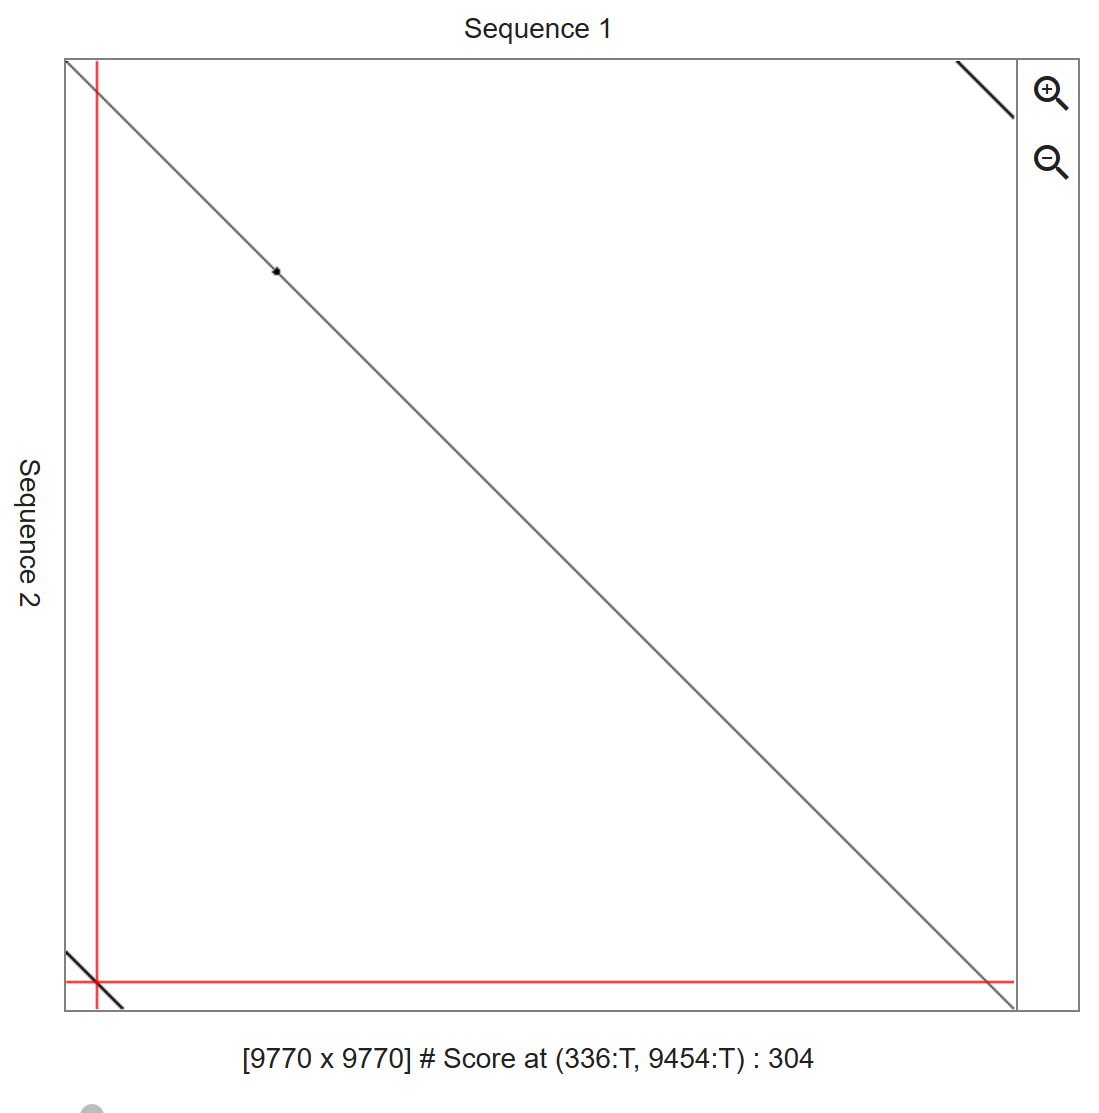
\includegraphics{dotplot.png}
\caption{dotplot.png}
\end{figure}

    From the dotplot above we can see that there are same segments of the
sequence at the beginning and at the end of the squence. This means that
there is a prefix of the sequence that is the same as the suffix. There
is also a repetitive segment at about 1/4 of the sequence.

We tried multiple settings of the dotplot but found no other interesting
patterns. However, there still may be some due to the fact that the
image must be higly compressed.

I used https://dotlet.vital-it.ch/ for generating and studying the
picture because the tool provided in the task was not accessable (403 -
Forbidden).


    % Add a bibliography block to the postdoc
    
    
    
    \end{document}
